\documentclass[article,12pt]{elsarticle}
\usepackage[spanish]{babel}
\usepackage[utf8]{inputenc}
\usepackage{amssymb}
\usepackage{flushend}
\usepackage{float}
\usepackage{anysize}
\usepackage{amsmath}
\usepackage{amsfonts}
\usepackage{dcolumn}
\usepackage{amsthm}
\usepackage{caption}
\usepackage{float}
\usepackage{subfigure}
\usepackage{graphicx}
\usepackage{lmodern}
\usepackage{booktabs}
\usepackage{color}
\usepackage{longtable}
\usepackage{rotating}
\usepackage{etoolbox}
\usepackage{comment}
\usepackage{pdflscape}
\usepackage{booktabs}
\usepackage[table,xcdraw]{xcolor}

\begin{document}

\begin{frontmatter}
    \title{Laboratorio de Electromagnetismo \\  Práctica  6\\ 
        Condensador de placas paralelas y dieléctricos}
    \author{Iván Bautista Alvarado$^1$ y Andrés López González$^1$} %Aquí va el nombre de los integrantes que participaron en el informe.
    \address{$^1$ Facultad de Ciencias, Universidad Nacional Autónoma de México, M\'exico CDMX.}


    \begin{abstract}
     This research investigates the fundamental principles of capacitors, specifically the determination of vacuum permittivity $\epsilon_0$ and dielectric constants of various insulating materials such as wood, acrylic, and glass. The study begins by revisiting the theoretical framework of parallel-plate capacitors, establishing the relationship between stored charge, capacitance, and the electric field. Through the application of dielectric materials within the capacitor, the effect on capacitance and electric field is explored, with an emphasis on how the permittivity of these materials alters the system's overall behavior.

Experimental measurements were conducted using a parallel-plate capacitor configuration, with capacitors of varying sizes and dielectric materials introduced between the plates. The capacitance was measured under different configurations, and the permittivity of the vacuum was estimated by analyzing the linear relationship between capacitance and plate separation for the different plate sizes. The results yielded an average vacuum permittivity of $(4.2125 \pm 28.35 \%) pF/m$ , which is approximately half the accepted value of $\epsilon_0 \approx 8.854 pF/m$. This significant discrepancy was attributed to mechanical imperfections in the parallel plate alignment and limitations in the precision of the setup.

Dielectric constants for the materials tested were determined by inserting them into the capacitor and observing changes in capacitance. The constants obtained were compared with established values, providing insight into the variability of dielectric behavior across different materials. While the precision of the measurements was affected by experimental limitations, the results highlight the importance of setup accuracy in high-precision electromagnetic experiments and suggest avenues for improving the alignment and stability of parallel-plate systems in future research.

Overall, this study provides a comprehensive analysis of capacitor behavior under varying conditions and offers experimental insights into the determination of material dielectric properties, with potential applications in the design and optimization of energy storage devices.
    \end{abstract}

    \begin{keyword}
     Capacitance; Dielectrics; Parallel Plate Capacitor; Electric Field; Permittivity
    \end{keyword}
\end{frontmatter}
\section*{Resumen}
Esta investigación investiga los principios fundamentales de los capacitores, específicamente la determinación de la permitividad del vacío \(\epsilon_0\) y las constantes dieléctricas de varios materiales aislantes como madera, acrílico y vidrio. El estudio comienza revisando el marco teórico de los capacitores de placas paralelas, estableciendo la relación entre la carga almacenada, la capacitancia y el campo eléctrico. A través de la aplicación de materiales dieléctricos dentro del capacitor, se explora el efecto sobre la capacitancia y el campo eléctrico, con énfasis en cómo la permitividad de estos materiales altera el comportamiento general del sistema.

Se realizaron mediciones experimentales utilizando una configuración de capacitores de placas paralelas, con capacitores de diferentes tamaños y materiales dieléctricos introducidos entre las placas. La capacitancia se midió bajo diferentes configuraciones y la permitividad del vacío se estimó analizando la relación lineal entre la capacitancia y la separación de placas para los diferentes tamaños de placas. Los resultados arrojaron una permitividad de vacío promedio de \((4.2125 \pm 28.35\%) \, \text{pF/m}\), que es aproximadamente la mitad del valor aceptado de \(\epsilon_0 = 8.854 \; pF/m \). Esta discrepancia significativa se atribuyó a imperfecciones mecánicas en la alineación de las placas paralelas y limitaciones en la precisión de la configuración.

Las constantes dieléctricas de los materiales probados se determinaron insertándolos en el condensador y observando los cambios en la capacitancia. Las constantes obtenidas se compararon con los valores establecidos, lo que proporcionó información sobre la variabilidad del comportamiento dieléctrico en diferentes materiales. Si bien la precisión de las mediciones se vio afectada por limitaciones experimentales, los resultados resaltan la importancia de la precisión de la configuración en experimentos electromagnéticos de alta precisión y sugieren vías para mejorar la alineación y la estabilidad de los sistemas de placas paralelas en futuras investigaciones.

En general, este estudio proporciona un análisis exhaustivo del comportamiento de los condensadores en distintas condiciones y ofrece conocimientos experimentales para la determinación de las propiedades dieléctricas del material, con posibles aplicaciones en el diseño y la optimización de dispositivos de almacenamiento de energía.

\noindent \textit{Palabras clave:}  Capacitancia; Dieléctricos; Capacitor de placas paralelas; Campo eléctrico; Permitividad

\section{Introducción}
    \textbf{Capacitores} \\
    Por definición, un capacitor consiste en dos densidades de cargas, con cargas netas opuestas, que generan un campo eléctrico de una de las densidades a la otra. La idea del capacitor es "almacenar" carga y energía. Para poder almacenar la energía se necesita del campo eléctrico, pues su potencial eléctrico asociado es el que nos va a permitir tener esa energía potencial almacenada. Al haber una distancia de separación y tener el capacitor en un medio aislante, como el aire, la diferencia de potencial no va a ser capaz de mover las cargas de un lado a otro (en principio). Y de esta manera las cargas van a quedar con una energía potencial. Como habíamos dicho, en principio, la diferencia de potencial no va a ser suficiente para que las cargas sean capaces de moverse por el medio aislante, esto nos permite suministrarle más carga a nuestras densidades de carga y así almacenar la carga. De esta manera se define la capacitancia de un capacitor:
    \begin{equation}
        C=\frac{q}{\Delta V}
    \end{equation}
    Donde q es la magnitud de la carga que se tiene en las densidades de carga, y $\Delta V$ es la diferencia de potencial que genera su campo eléctrico. C es la capacitancia y mide la capacidad de almacenar carga.\\

    \textbf{Condensador de placas paralelas}\\
    El capacitor más sencillo de estudiar y analizar son dos placas paralelas de un material conductor, a los que se le suministra carga.
    Al ser dos placas paralelas cargadas (opuestamente) su campo eléctrico es uniforme y viene dado por:
    \begin{equation}
        E = \frac{q}{A \epsilon_0}
    \end{equation}
    Donde A es el area transversal de las placas.
    Con esto, es fácil la diferencia de potencial que se genera:
    \begin{equation}
        \Delta V = -Ed
    \end{equation}
    Donde d es la distancia de separacion de las placas
    Con estas dos ecuaciones podemos obtener $\epsilon_0$ , pues
    \begin{equation*}
        C = \frac{\epsilon_0 A}{d} 
    \end{equation*}
    \begin{equation}
        \epsilon_0 = \frac{Cd}{A}
    \end{equation}\\
    
    \textbf{Dieléctricos}\\
    Un dieléctrico es un material que se coloca en medio del capacitor, con la finalidad de aumentar la capacitancia. Esto solo lo pueden cumplir los materiales aislantes, pues los conductores o semiconductores pueden permitir el paso de las cargas y el capacitor terminaría por descargarse. 
    Dentro del material aislante, se genera otro campo eléctrico dentro del material dieléctrico con sentido opuesto al campo eléctrico del capacitor como se muestra en la figura:
    \begin{figure}[H]
        \centering
        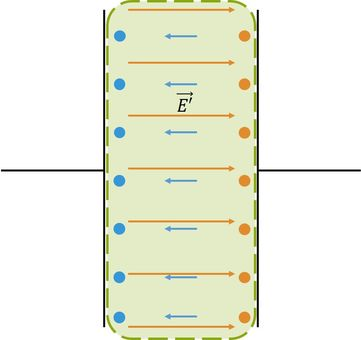
\includegraphics[width=0.5\linewidth]{Dielectrico.png}
        \caption{Campo eléctrico dentro de un dieléctrico. Imagen obtenida de: https://www.calculisto.com/}
    \end{figure}
    de esta manera, al ser opuestos, el campo total es menor al inicial y su diferencia de potencial también es menor $\Delta V_i >\Delta V_f$. Entonces por la ec 1. tenemos que $C_i<C_f$.\\

    Estos materiales dieléctricos tienen una permitividad $\epsilon$ distinta a la del vacío. Así definimos a la constante dieléctrica de un material (o permitividad relativa):
    \begin{equation*}
        \kappa = \frac{\epsilon}{\epsilon_0}
    \end{equation*}
    \textbf{Conexión en serie de capacitores}
    Para una conexión en serie, la capacitancia de los capacitores se suman como los inversos de cada uno:
    \begin{equation}
        \frac{1}{C_T} = \sum_i \frac{1}{C_i}
    \end{equation}
    Cuando hay solo un capacitor con dieléctrico:
    \begin{equation*}
        \frac{1}{C_T} = \frac{1}{\frac{\epsilon A}{d}} = \frac{d}{\epsilon A}
    \end{equation*}
    \begin{equation}
        C_T= \frac{\epsilon A}{d}
    \end{equation}
    \begin{equation}
        \Rightarrow \epsilon = \frac{d C_T}{A}
    \end{equation}
    Así, sabiendo la capacitancia total, y la forma ,con sus dimensiones, del dieléctrico, podemos obtener la permitividad del material y con la ec. 5 su constante dieléctrica.
    \subsection{Hipótesis}
    Esperamos obtener un resultado similar a la permitividad del vacío, que se ha determinado experimentalmente como: $\epsilon_0 \approx 8.8541878176 \cdot 10^{-12}$ F/m.

    Y las constantes dieléctricas deben de ser de:
    \begin{table}[H]
    \begin{center}
\begin{tabular}{|c|c|}
\hline
Madera   & 1.4$\rightarrow$6.0  \\ \hline
Acrílico & 1.6$\rightarrow$4.0  \\ \hline
Vidrio   & 5.0$\rightarrow$8.0 \\ \hline
\end{tabular}
\end{center}
\end{table}
    \subsection{Objetivos}
    Determinar la permitividad del vacío, y determinar la constante dieléctrica de distintos materiales.

\section{Desarrollo Experimenal / Métodos}
Materiales utilizados:
    \begin{itemize}
        \item 1 Medidor de capacitancia
        \item 1 Condensador de placas paralelas
        \item 3 Pares de discos de aluminio de diferentes tamaños
        \item 3 Discos de madera de diferentes tamaños
        \item 3 Discos de acrílico de diferentes tamaños
        \item 3 Discos de vidrio de diferentes tamaños
        \item 2 Cables banana-banana
        \item 1 Vernier
        \item Masking Tape
        \item 1 Fuente de poder
    \end{itemize}
    El experimento consiste en montar el condensador de placas paralelas con los pares de discos de aluminio con el mismo tamaño, se deben de acercar las placas sin tocarse a una distancia pequeña, y después conectar el condensador a la fuete de poder para suministrar electricidad. Se mide la capacitancia con el medidor de capacitancia y se registra su capacitancia a esa distancia. Después se cambia la distancia de la placas y se vuelve a medir la capacitancia y la distancia. Esto se hace al menos 10 veces para ese par de discos. Luego se cambia el par de discos y se repiten las mediciones de la misma manera.
    
    Ahora se introduce un disco de madera entre las placas con los discos de aluminio, el radio del disco de madera debe procurarse lo más parecido al radio de los discos de aluminio que se estén usando, y las placas deben pegadas al disco de madera, se enciende la fuente de poder conectada al condensador, y se mide la capacitancia.
    Después se cambia el tamaño del disco de madera que se va a introducir entre las placas, y si es necesario, se cambian los discos de aluminio para que el radio sea lo más parecido al nuevo disco de madera. Nuevamente se juntan lo más posible, se enciende la fuente y se mide la capacitancia.
    Esto se hace para el resto de discos de madera, vidrio y acrílico.

    También deben medirse los radios de los discos para conocer sus areas transversales. Y en el caso de los discos de madera, vidrio y acrílico debe de medirse también su grosor.
    
    Es importante que las placas estén lo más paralelas y alineadas posibles, en el caso de los dieléctricos se puede usar masking tape para fijar las placas.
\section{Resultados y discusión}
Para la primera parte del capacitor de distintos radios, obtuvimos las siguientes tabla.
\begin{table}[H]
\centering
\begin{tabular}{|c|c|}
\hline
\rowcolor[HTML]{C0C0C0} 
\textbf{1/s (1/m)}                 & \textbf{Capacitancia (pF)}              \\ \hline
\rowcolor[HTML]{FFFFFF} 
{\color[HTML]{000000} 1,000.00}    & {\color[HTML]{000000} 0.0000000000479} \\ \hline
\rowcolor[HTML]{FFFFFF} 
{\color[HTML]{000000} 500.00}      & {\color[HTML]{000000} 0.0000000000363} \\ \hline
\rowcolor[HTML]{FFFFFF} 
{\color[HTML]{000000} 333.33}      & {\color[HTML]{000000} 0.0000000000316} \\ \hline
\rowcolor[HTML]{FFFFFF} 
{\color[HTML]{000000} 250.00}      & {\color[HTML]{000000} 0.0000000000277} \\ \hline
\rowcolor[HTML]{FFFFFF} 
{\color[HTML]{000000} 200.00}      & {\color[HTML]{000000} 0.0000000000253} \\ \hline
\rowcolor[HTML]{FFFFFF} 
{\color[HTML]{000000} 166.67}      & {\color[HTML]{000000} 0.0000000000233} \\ \hline
\rowcolor[HTML]{FFFFFF} 
{\color[HTML]{000000} 142.86}      & {\color[HTML]{000000} 0.0000000000225} \\ \hline
\rowcolor[HTML]{FFFFFF} 
{\color[HTML]{000000} 125}         & {\color[HTML]{000000} 0.0000000000215} \\ \hline
\rowcolor[HTML]{FFFFFF} 
{\color[HTML]{000000} 111.1111111} & {\color[HTML]{000000} 0.0000000000209} \\ \hline
\rowcolor[HTML]{FFFFFF} 
{\color[HTML]{000000} 100}         & {\color[HTML]{000000} 0.0000000000204} \\ \hline
\end{tabular}
\caption{Tabla para primer par de placas paralelas de radio $4.95cm \pm \frac{mm}{20}$}
\end{table}
Obtenemos que, al calcular la pendiente capacitancia vs tiempo del primer par de placas paralelas ($3.1026 \cdot 10^{-14}$) y dividirla entre el área de cada placa paralela, el resultado es de $(4.031 \pm 29.0752\%)\frac{pF}{m}$, quien justamente es la permitividad del vacío. Esto de acuerdo a la evidencia científica no es verdad, pues la permitividad del vacío es de $8.8541878176 \frac{pF}{m}$ y en el aire esta es demasiado similar. Este defecto es mucho más del 0.29\% que nos reportó la propagación de incertidumbres, del mismo modo no pudo haber influenciado el aire al tener una permitividad bastante similar, por lo cual atribuimos este defecto al montaje de placas paralelas ya que existían errores mecánicos en este arreglo, lo cual nos impedía tener las placas totalmente paralelas a pesar de ajustarlo lo mejor posible mediante papel.

\begin{table}[H]
\centering
\begin{tabular}{|c|c|}
\hline
\rowcolor[HTML]{C0C0C0} 
\textbf{1/s (1/m)}                 & \textbf{Capacitancia (pF)}              \\ \hline
\rowcolor[HTML]{FFFFFF} 
{\color[HTML]{000000} 1,000.00}    & {\color[HTML]{000000} 0.0000000001215} \\ \hline
\rowcolor[HTML]{FFFFFF} 
{\color[HTML]{000000} 500.00}      & {\color[HTML]{000000} 0.0000000000950} \\ \hline
\rowcolor[HTML]{FFFFFF} 
{\color[HTML]{000000} 333.33}      & {\color[HTML]{000000} 0.0000000000706} \\ \hline
\rowcolor[HTML]{FFFFFF} 
{\color[HTML]{000000} 250.00}      & {\color[HTML]{000000} 0.0000000000528} \\ \hline
\rowcolor[HTML]{FFFFFF} 
{\color[HTML]{000000} 200.00}      & {\color[HTML]{000000} 0.0000000000470} \\ \hline
\rowcolor[HTML]{FFFFFF} 
{\color[HTML]{000000} 166.67}      & {\color[HTML]{000000} 0.0000000000438} \\ \hline
\rowcolor[HTML]{FFFFFF} 
{\color[HTML]{000000} 142.86}      & {\color[HTML]{000000} 0.0000000000409} \\ \hline
\rowcolor[HTML]{FFFFFF} 
{\color[HTML]{000000} 125}         & {\color[HTML]{000000} 0.0000000000380} \\ \hline
\rowcolor[HTML]{FFFFFF} 
{\color[HTML]{000000} 111.1111111} & {\color[HTML]{000000} 0.0000000000346} \\ \hline
\rowcolor[HTML]{FFFFFF} 
{\color[HTML]{000000} 100}         & {\color[HTML]{000000} 0.0000000000327} \\ \hline
\end{tabular}
\caption{Tabla para el segundo par de placas paralelas de radio $8.75cm \pm \frac{mm}{20}$}
\end{table}

Para el segundo par de placas paralelas obtenemos el siguiente valor para la permitividad del vacío: $(4.2765 \pm 28.1394\%)\frac{pF}{m}$, es bastante similar a nuestro cálculo anterior pero nuevamente difiere de la permitividad del vacío por el doble, aunque se mantiene en el mismo orden numérico.

\begin{table}[H]
\centering
\begin{tabular}{|c|c|}
\hline
\rowcolor[HTML]{C0C0C0} 
\textbf{1/s (1/m)}                 & \textbf{Capacitancia (pF)}             \\ \hline
\rowcolor[HTML]{FFFFFF} 
{\color[HTML]{000000} 1,000.00}    & {\color[HTML]{000000} 0.0000000001942} \\ \hline
\rowcolor[HTML]{FFFFFF} 
{\color[HTML]{000000} 500.00}      & {\color[HTML]{000000} 0.0000000001381} \\ \hline
\rowcolor[HTML]{FFFFFF} 
{\color[HTML]{000000} 333.33}      & {\color[HTML]{000000} 0.0000000001243} \\ \hline
\rowcolor[HTML]{FFFFFF} 
{\color[HTML]{000000} 250.00}      & {\color[HTML]{000000} 0.0000000000818} \\ \hline
\rowcolor[HTML]{FFFFFF} 
{\color[HTML]{000000} 200.00}      & {\color[HTML]{000000} 0.0000000000713} \\ \hline
\rowcolor[HTML]{FFFFFF} 
{\color[HTML]{000000} 166.67}      & {\color[HTML]{000000} 0.0000000000630} \\ \hline
\rowcolor[HTML]{FFFFFF} 
{\color[HTML]{000000} 142.86}      & {\color[HTML]{000000} 0.0000000000582} \\ \hline
\rowcolor[HTML]{FFFFFF} 
{\color[HTML]{000000} 125}         & {\color[HTML]{000000} 0.0000000000536} \\ \hline
\rowcolor[HTML]{FFFFFF} 
{\color[HTML]{000000} 111.1111111} & {\color[HTML]{000000} 0.0000000000498} \\ \hline
\rowcolor[HTML]{FFFFFF} 
{\color[HTML]{000000} 100}         & {\color[HTML]{000000} 0.0000000000470} \\ \hline
\end{tabular}
\caption{Tabla para el tercer par de placas paralelas de radio $11.15cm \pm \frac{mm}{20}$}
\end{table}

Para nuestro último par de placas paralelas la permitividad del vacío es de $(4.3301 \pm 27.840\%)pF$, muy similar a los anteriores y mismo comentario. Por lo que finalmente nuestro promedio fue que la permitividad del vacio es de $(4.2125 \pm 28.3516)\frac{pF}{m}$, siendo bastante constante este valor para cada radio y aunque se aleja ligeramente de la permitividad reportada experimentalmente del vacío, mantenemos un número del mismo orden.\\\\

Para la segunda parte del experimento, obtuvimos las siguientes tablas en donde medimos el grosor de un dieléctrico, su capacitancia y área superficial.

\begin{table}[H]
\centering
\begin{tabular}{ccc}
\hline
\multicolumn{1}{|c|}{Separación de la madera (m) $\pm$ mm/20} & \multicolumn{1}{c|}{Capacitancia (F)}  & \multicolumn{1}{c|}{Area disco gigante} \\ \hline
\multicolumn{1}{|c|}{0.017500000}                              & \multicolumn{1}{c|}{0.000000000032810} & \multicolumn{1}{c|}{0.0390570652676}    \\ \hline
                                                               &                                        &                                         \\ \hline
\multicolumn{1}{|c|}{Separación de la madera (m) $\pm$ mm/20} & \multicolumn{1}{c|}{Capacitancia (F)}  & \multicolumn{1}{c|}{Area disco mediano} \\ \hline
\multicolumn{1}{|c|}{0.005200000}                              & \multicolumn{1}{c|}{0.000000000051923} & \multicolumn{1}{c|}{0.02405281875}      \\ \hline
                                                               &                                        &                                         \\ \hline
\multicolumn{1}{|c|}{Separación de la madera (m) $\pm$ mm/20} & \multicolumn{1}{c|}{Capacitancia (F)}  & \multicolumn{1}{c|}{Area disco pequeño} \\ \hline
\multicolumn{1}{|c|}{0.003275000}                              & \multicolumn{1}{c|}{0.000000000029129} & \multicolumn{1}{c|}{0.007697687399}     \\ \hline
\end{tabular}
\caption{Tabla de datos para la madera como dieléctrico}
\end{table}

Al analizar estos datos deducimos que la permitividad del material para cada uno de los tamaños del dieléctrico (en este caso la madera) es $1.4701 \cdot 10^{-11} \frac{F}{m}$ para el capacitor pequeño, $1.1225 \cdot 10^{-11} \frac{F}{m}$ para el capacitor mediano y $1.2393 \cdot 10^{-11}\frac{F}{m}$ para el grande. Obteniendo que la permitividad de la madera es de $1.2773 \cdot 10^{-11} \pm 59.0652\%$, además al considerar la permitividad del vacío real obtuvimos que la permitividad relativa (constante dieléctrica) es $1.5966 \pm 59.0652 \%$; no pudimos obtener un dato de comparación conciso para los dieléctricos pues las diferentes fuentes indican que la constante dieléctrica puede variar mucho en función de la estructura química del trozo de madera, pero está en el rango de $1.4\rightarrow 6.0$ que hemos encontrado.

\begin{table}[H]
\centering
\begin{tabular}{ccl}
\hline
\multicolumn{1}{|c|}{Separación del acrílico (m) $\pm$ 1/20mm} & \multicolumn{1}{c|}{Capacitancia (F)}  & \multicolumn{1}{l|}{Area disco gigante} \\ \hline
\multicolumn{1}{|c|}{0.010000000}                              & \multicolumn{1}{c|}{0.000000000054868} & \multicolumn{1}{r|}{0.0390570652676}    \\ \hline
\multicolumn{1}{l}{}                                           & \multicolumn{1}{l}{}                   &                                         \\ \hline
\multicolumn{1}{|c|}{Separación del acrílico (m) $\pm$ 1/20mm} & \multicolumn{1}{c|}{Capacitancia (F)}  & \multicolumn{1}{l|}{Area disco mediano} \\ \hline
\multicolumn{1}{|c|}{0.006050000}                              & \multicolumn{1}{c|}{0.000000000076317} & \multicolumn{1}{c|}{0.02405281875}      \\ \hline
\multicolumn{1}{l}{}                                           & \multicolumn{1}{l}{}                   &                                         \\ \hline
\multicolumn{1}{|c|}{Separación del acrílico (m) $\pm$ 1/20mm} & \multicolumn{1}{c|}{Capacitancia (F)}  & \multicolumn{1}{l|}{Area disco pequeño} \\ \hline
\multicolumn{1}{|c|}{0.003120000}                              & \multicolumn{1}{c|}{0.000000000035651} & \multicolumn{1}{r|}{0.007697687399}     \\ \hline
\end{tabular}
\caption{Tabla de datos para el acrílico como dieléctrico}
\end{table}

La permitividad en este caso del acrílico es $1.4048 \cdot 10^{-11} \frac{F}{m}$ para el capacitor pequeño, $1.9196 \cdot 10^{-11} \frac{F}{m}$ para el capacitor mediano y $1.4450 \cdot 10^{-11}\frac{F}{m}$ para el grande. Deduciendo que la permitividad del acrílico es de $1.5898 \cdot 10^{-11} \pm 79.1463\%$, y su permitividad relativa (constante dieléctrica) es $1.9873E \pm 79.1463 \%$. En este caso la permitividad relativa está muy cerca a la esperada según el marco teórico ($1.6 \rightarrow 4.0$).

\begin{table}[H]
\centering
\begin{tabular}{ccl}
\hline
\multicolumn{1}{|c|}{Separación del vidrio (m) $\pm$ 1/20mm} & \multicolumn{1}{c|}{Capacitancia (F)}  & \multicolumn{1}{l|}{Area disco gigante} \\ \hline
\multicolumn{1}{|c|}{0.005375000}                            & \multicolumn{1}{c|}{0.000000000382000} & \multicolumn{1}{r|}{0.0390570652676}    \\ \hline
\multicolumn{1}{l}{}                                         & \multicolumn{1}{l}{}                   &                                         \\ \hline
\multicolumn{1}{|c|}{Separación del vidrio (m) $\pm$ 1/20mm} & \multicolumn{1}{c|}{Capacitancia (F)}  & \multicolumn{1}{l|}{Area disco mediano} \\ \hline
\multicolumn{1}{|c|}{0.006050000}                            & \multicolumn{1}{c|}{0.004760000}       & \multicolumn{1}{c|}{0.000000000234000}  \\ \hline
\multicolumn{1}{l}{}                                         & \multicolumn{1}{l}{}                   &                                         \\ \hline
\multicolumn{1}{|c|}{Separación del vidrio (m) $\pm$ 1/20mm} & \multicolumn{1}{c|}{Capacitancia (F)}  & \multicolumn{1}{l|}{Area disco pequeño} \\ \hline
\multicolumn{1}{|c|}{0.003120000}                            & \multicolumn{1}{c|}{0.003180000}       & \multicolumn{1}{c|}{0.000000000067000}  \\ \hline
\end{tabular}
\caption{Tabla de datos para el vidrio como dieléctrico}
\end{table}

Finalmente obtenemos que la permitividad para el vidrio es $5.2571 \cdot 10^{-11} \frac{F}{m}$ para el capacitor pequeño, $4.6308E \cdot 10^{-11} \frac{F}{m}$ para el capacitor mediano y $2.7678E \cdot 10^{-11}\frac{F}{m}$ para el grande. Se calculó así que la permitividad del vidrio es de $4.2186E \cdot 10^{-11} \pm 112.8745\%$, el porcentaje de incertidumbre nos ha parecido demasiado alto en este caso pero debido a la magnitud de nuestras capacitancias la propoagación de incertidumbres fue inducida de esta manera. Y su permitividad relativa es $5.2732 \pm 112.8745 \%$. En este caso la permitividad relativa central está rozando a la permitividad esperada ($5.0\rightarrow 8.0$), pero nos sigue pareciendo un dato bastante certero.

\section{Conclusiones}
En este trabajo se realizó un estudio experimental sobre la permitividad del vacío utilizando un condensador de placas paralelas y diversos materiales dieléctricos. Los resultados obtenidos permiten validar el comportamiento esperado del capacitor, aunque se observan discrepancias significativas entre los valores obtenidos y la permitividad teórica del vacío, \(\epsilon_0 = 8.854 \; pF/m\). Las mediciones experimentales arrojaron un valor promedio de la permitividad del vacío de \((4.2125 \pm 28.35)\, \text{pF/m}\), lo que representa una desviación importante de más del $50\%$ con respecto al valor teórico. Atribuimos estas discrepancias principalmente a los errores mecánicos durante el montaje experimental, especialmente la dificultad para alinear perfectamente las placas paralelas, lo que pudo haber influido en el campo eléctrico generado entre ellas y, en consecuencia, en la capacitancia medida.

En la segunda parte del experimento, se introdujeron diversos materiales dieléctricos como madera, acrílico y vidrio. Como era de esperarse, al colocar estos materiales entre las placas, la capacitancia aumentó debido a la presencia de un campo eléctrico inducido que redujo el campo neto del condensador, permitiendo almacenar más carga por la misma diferencia de potencial. Los valores de las constantes dieléctricas obtenidos estuvieron en el rango teórico de cada material, lo que valida el comportamiento predicho para sistemas capacitivos con dieléctricos.

A pesar de las limitaciones y errores observados, el experimento cumple con el objetivo de demostrar el principio básico de los capacitores y la influencia de los dieléctricos en la capacitancia. Para futuras investigaciones, se recomienda mejorar la precisión del montaje experimental, especialmente en la alineación de las placas, y considerar la influencia de factores externos como el aire y la temperatura, que podrían afectar las mediciones. Además, sería de interés profundizar en la investigación del montaje de más de un dieléctrico para observar la interacción entre el campo eléctrico y diferentes medios materiales.

\newpage
\noindent {\bf Declaración de contribución de los autores}\\ 

Iván Bautista Alvarado$^1$ y Andrés López González$^1$ hemos realizado tanto el apartado escrito como el análisis de manera colectiva siendo una participación del 100\% por parte de ambos y no solo una repartición.\\ 

{\bf Agradecimientos} \\ 

A ese.\\

\begin{figure}[h]
    \centering
    
\includegraphics[width=0.5\linewidth]{el.png}
    \caption{Electrogato}
    \label{fig:enter-label}
\end{figure}\\

\begin{thebibliography}{99}

\bibitem{griffiths}
D. J. Griffiths, \textit{Introduction to Electrodynamics}, 3rd ed. Upper Saddle River, NJ, USA: Prentice-Hall, 1999.

\bibitem{jackson}
J. D. Jackson, \textit{Classical Electrodynamics}, 3rd ed. New York, NY, USA: Wiley, 1998.

\bibitem{sadiku}
M. N. O. Sadiku, \textit{Elements of Electromagnetics}, 6th ed. New York, NY, USA: Oxford University Press, 2014.

\bibitem{wangsness}
R. K. Wangsness, \textit{Electromagnetic Fields}, 2nd ed. New York, NY, USA: Wiley, 1986.

\bibitem{zangwill}
A. Zangwill, \textit{Modern Electrodynamics}. Cambridge, UK: Cambridge University Press, 2013.

\bibitem{purcell}
E. M. Purcell and D. J. Morin, \textit{Electricity and Magnetism}, 3rd ed. Cambridge, UK: Cambridge University Press, 2013.

\bibitem{shadowitz}
A. Shadowitz, \textit{The Electromagnetic Field}. Mineola, NY, USA: Dover Publications, 1988.


\end{thebibliography}


\end{document}